\documentclass[12pt]{article}

\usepackage{amsmath}
\usepackage{graphicx}
\usepackage{listings}
\usepackage{graphicx}
\usepackage{caption} 
\usepackage[linkcolor=black,citecolor=red,urlcolor=cyan,colorlinks=true]{hyperref}

\title{\textsc{Report for 1DV516\\\large{Algorithms and Advanced Data Structures}}}
\author{\textsc{Ingmar Immanuel Falk}}
\date{\textsc{\today}}

\begin{document}

\maketitle
\pagebreak
\tableofcontents
\pagebreak

\section{Abstract}
This report will go over how I solved the problems in the assignment.

\section{Introduction}

In this report I will elaborate my solutions to the required problems (4-7) as well
as the problems for the grade VG (8).
I will start with a general description of the setup for the experiments, how I tested
my algorithms for both correctness and speed and how I then used those results to 
create visualizations of the data.

\section{Experiment Setup}

Before I will go into the details of the testing, benchmarking and visualizations. I will elaborate
the general structure of the project and the code. 

\subsection{Structure}

I have structured the project so that every major responsibility is contained within its 
own folder.

\texttt{bencharks} contains all benchmarking code

\texttt{bench\_results} contains all benchmarking results as \emph{.csv} files

\texttt{tests} contains all the testing code

\texttt{analysis} contains all the python code for data analysis

\texttt{fits} contains all the plots with fitted graphs generated using \emph{scipy}

\texttt{calcs} contains all the results for the fits generated using \emph{scipy} 

\texttt{plots} contains all the generated visualizations as \emph{.png} files

\texttt{bin} contains the compiled java code

\texttt{src} contains all the source code for the algorithms as well as the helper utility
for the testing and benchmarking

Running any functionality of the project should be done via \emph{make}. The \emph{Makefile}
is located in the root of the project and contains all the necessary commands to build the java code,
run tests and benchmarks and generate the visualizations.

\subsection{Testing}

To test the correctness of the algorithms I have created a couple of helper classes that
allow me to string together a series of tests and then run them. The results are printed
to \emph{stdout} and contain information about which tests passed and which failed. The 
Makefile contains commands to run all tests together or just a single file. Its not very
advanced but it is enough for the purpose of this assignment.

My tests were simple, I took small inputs for which I could figure out the supposed
output myself and used it to test the algorithms. For some algorithms I added more tests, just
to be sure, because while the algorithms are fairly trivial to implement, the improved cache
version required slightly more thinking. But I will talk more about that later in \hyperlink{p5}{Problem 5} and \hyperlink{p6}{Problem 6}. 

\subsection{Benchmarking}

For the benchmarking I did something similar and created a set of utility classes that use Java's
\emph{System.nanoTime()} to measure the time it takes to run a given algorithm. To make the 
\emph{bench} function I used for all my tests generic, I this public interface:

\begin{lstlisting}[language=Java]
    public <T> void bench(
        String name, 
        String filename,
        Function<Integer, T> setup,
        Consumer<T> fn,
        List<Integer> sizes,
        int reps
    ) { ... }
\end{lstlisting}


The parameters \emph{name} and \emph{filename} are quite trivial and simply used to display the name
of the benchmark to \emph{stdout} and to save the results to a \emph{.csv} file. The rest requires some more explanation:

\begin{itemize}
    \item \emph{setup} takes the size to test an arbitrary algorithm at as input and returns the algorithms input as type \emph{T}. This is so that the setup can be adjusted according to the size. It is also crucial to our ability to make the benchmarks multithreadable. This setup function allows us to isolate each thread and encapsulate everything it needs so we dont have any shared state.
    \item \emph{fn} is a function that takes the input generated by the \emph{setup} of type \emph{T} as input and returns nothing. This function is the algorithm that is being benchmarked.
    \item \emph{sizes} is a list of integers that represent the input sizes that should be benchmarked. The benchmarking function will run the algorithm for each input size and measure the time it takes to run the algorithm for each input size.
    \item \emph{reps} is the number of times the algorithm should be run for each input size. The benchmarking function will run the algorithm \emph{reps} times for each input size and then calculate the average time it took to run the algorithm for each input size.
\end{itemize}

While we get the time as \emph{nano seconds}, we store and display it in \emph{milli seconds} to make it easier to read.

\subsection{Visualizations}

For the visualizations I used \emph{python} and \emph{matplotlib}, \emph{numpy} and \emph{scipy}. There is not much to say here.
I simply load the data using numpy and then pass use it with matplotlib to generate simple graphs. For the fitting I used scipy's \emph{curve\_fit} function
together with a couple of simple functions I defined such as linear, quadratic, cubic etc..

\section{Problems - G}


\subsection{Problem 4 - UnionFind Benchmarking \& Growth}

For the comparison between the basic Quick Find version of Union Find and some improved version,
I chose the Weighted Quick Union \emph{(WQU)}. And although I also implemented all other
options, I will only use the results for the \emph{WQU} implementation for the comparison.

\subsubsection{Quick Union Expectations}

Before looking at the benchmarks and calculations we need to think about what we expect to 
be able to check if we messed up our implementation or if it was correct.

The dominant factor when to consider when arguing about the runtime performance of the 
basic quick find implementation is the \emph{union} function and here in particular the 
\emph{for loop} over all \emph{N} elements. This will obviously result in a time complexity
of \emph{O(N)} as other operations such as retreiving the id/root are \emph{O(1)} operations
and since we ignore lower order terms and coefficients that leaves us with \emph{O(N)}.

\subsubsection{Weighted Quick Union Expectations}

For the \emph{WQU} however we expect something quite a bit better than \emph{O(N)}. The reason
for this is the check we perform in every union. We maintain a list of weights for all nodes,
and with every union, the weight of the two nodes to be connected will be compared and the 
node that has a lower weight will be appended to the heavier one. I am using weight instead
of size as this name more accurately describes what we are keeping track of here. Since we
are only keeping track of the total number of nodes in one tree, not the depth/size of it.
For a list of length N we could have a single union with weight N but a max depth of 1.

Now the reason this check will give us a huge performance boost is because now, the depth
of the tree can only be increased when two unions of the same size are connected together.
This means that in order to get the max depth of the tree, we would have to only ever 
unionise nodes with the same weight, which is equivalent to doubling the weight of all
nodes before moving on to the next round an doing the same thing again. Lets look at an example:

Lets start with a newly initialised list of size 8. We have 8 root nodes with a weight of 1
[(0, 1), (1, 1), (2, 1), (3, 1), (4, 1), (5, 1), (6, 1), (7, 1)]. In the first round, we unionise
4 unique pairs. This will result in 4 root nodes with a weight of 2
[(1, 1), (1, 2), (3, 1), (3, 2), (5, 1), (5, 2), (7, 1), (7, 2)]. By this point, the max 
depth is 1. The next iteration will result in 2 root nodes with a weight of 4 and a max depth of 2 and the last 
iteration last in one root node with a weight of 8 and a max depth of 3. At this point its weight is equal to N, 
since all of the nodes within the list have it as its root node. 

\pagebreak

If we want to apply this to any generic list of size N, we have to think about how many
of those iterations can we possibly do. This is the same as asking, how many times can we \emph{half}
the number of \emph{N} root nodes or how many times we can double 1. Both of these will
lead to the same result, which is \emph{$log_2 N$}. This holds not only for lengths of a power of 2,
but for any N, since in those cases the depth is still dominated by the largest power of 2 that is 
smaller than N.

All of this should lead uf to the expectation that the \emph{find} or \emph{root} function of
the Weighted Quick Union Find should have a time complexity of \emph{O(log N)}. If we think about
the time complexity of the \emph{union} and \emph{connected} function, where we have to call find/root
twice, it might seem like the time complexity should be \emph{O(2log N)} but since we ignore coefficients
this will still result in \emph{O(log N)} for both functions.

\subsubsection{Quick Union Results}

The benchmarking for the basic quick find implementation was done by running the \emph{union} function
on a list of \emph{N} sizes ranging from $10.000$ to $1.000.000$ in steps of $10.000$. Each function will be called $1.000$ times.
 The resulting growth we can observe is as expected linear. To facilitate this lets take a couple of points to calculate
the necessary values. For this 

\begin{table}[h]
    \centering
    \begin{tabular}{|c|c|c|c|c|c|c|c|}
        \hline size &	time &	l2 t &	ratio &	l2 r &	slope &	b &	c \\
        \hline 100000 &	15 &	3.95 &	N/A &	N/A &	N/A &	    N/A&	N/A \\
        \hline 200000 &	27 &	4.78 &	1.77 &	0.83 &	0.000120 &	0.826 &	-9.76 \\
        \hline 300000 &	44 &	5.49 &	1.63 &	0.71 &	0.000170 &	1.208 &	-16.50 \\
        \hline 400000 &	59 &	5.89 &	1.32 &	0.40 &	0.000145 &	0.972 &	-12.20 \\
        \hline 500000 &	72 &	6.19 &	1.23 &	0.30 &	0.000136 &	0.923 &	-11.28 \\
        \hline 600000 &	87 &	6.45 &	1.20 &	0.26 &	0.000144 &	0.991 &	-12.58 \\
        \hline 700000 &	104 &	6.71 &	1.20 &	0.26 &	0.000175 &	1.188 &	-16.36 \\
        \hline 800000 &	114 &	6.85 &	1.10 &	0.13 &	0.000102 &	0.695 &	-6.78 \\
        \hline 900000 &	132 &	7.05 &	1.15 &	0.20 &	0.000171 &	1.179 &	-16.28 \\
        \hline \multicolumn{2}{|c|}{average} & 6.17  &	1.33 &	0.39 &	0.000146 &	0.998 &	-12.72 \\
        \hline
    \end{tabular}
    \caption{\small{All the results of calculations based on the \emph{size} and \emph{time}. \emph{l2 t} = \emph{$log_2 time$}, \emph{l2 r} = \emph{$log_2 ratio$}}}
\end{table}

The \emph{size} and \emph{time} column are quite obvious to understand. The \emph{$log_2 t$} column contains
simply the $log_2$ of the original time values for comparing the values we get from our calculated
function and confirming its correctness. The same goes for the \emph{ratio/$log_2 ratio$} columns.
To calculate the slope we take the size and time of two rows and put them in this formula:
$\frac{time1 - time2}{size1 - size2}$. The \emph{$log_2 slope$} is basically the same but instead
of taking the raw values we use the $log_2$ of them, like this $\frac{log_2 time1 - log_2 time2}{log_2 size1 - log_2 size2}$.
Once we have the \emph{b}, we can use it to calculate the constant \emph{c} like this:
\emph{$c = log_2 time - b * log_2 size$}.
The reason why there are no values in the first row is that since we rely on the previous value for 
all results and there are no previous values for the first row, we are unable to calculate anything.

But now that we calculated the \emph{b} and \emph{c} for some points, we can take the average and use 
that to create a mode that predicts/approximates the \emph{$log_2$ of a time} for a given size. The function
in question looks like this \emph{$log_2 t = b * log_2 n + c$}, where t is the time and n the size. In our case,
the average \emph{b} is \emph{0.998} and the average \emph{c} is \emph{-12.72}, which leaves us with the 
following function: \emph{$log_2 t = 0.998 * log_2 n - 12.72$}. Lets compare the values we get from the model 
predictions to the original values.

\begin{table}[h]
    \centering
    \begin{tabular}{|c|c|c|c|}
        \hline size & original $log_2t$ & prediction & accuracy \\
        \hline 200000 & 4.78 & 4.85 & 0.98 \\
        \hline 300000 & 5.49 & 5.44 & 1.01 \\
        \hline 400000 & 5.89 & 5.85 & 1.01 \\
        \hline 500000 & 6.19 & 6.17 & 1.00 \\
        \hline 600000 & 6.45 & 6.43 & 1.00 \\
        \hline 700000 & 6.71 & 6.66 & 1.01 \\
        \hline 800000 & 6.85 & 6.85 & 1.00 \\
        \hline 900000 & 7.05 & 7.02 & 1.00 \\
        \hline
    \end{tabular}
    \caption{\small{Model Predictions vs Original $log_2$ times calculated with \emph{b} and \emph{c}}}
\end{table}

As we can see, the model predictions are quite accurate, with only minimal errors in their accuracy.
But these are only the $log_2$ values, to get the actual time we have to create a power law that approximates the actual time rather 
than just the $log_2$ of it. This is done by simply taking the already calculated \emph{b} and \emph{c} values and
plugging them into the general power law formula \emph{$a * x^b$}, where \emph{$a = 2^c$}. This results in the following
function: \emph{$t = 2^{-12.72} * n^{0.998}$} or \emph{$t = 0.00015 * n^{0.998}$}. Lets compare the values we get from the model predictions to the original values:

\begin{table}[h]
    \centering
    \begin{tabular}{|c|c|c|c|}
        \hline size & original t & prediction & accuracy \\
        \hline 100000 & 15.49 & 14.47 & 1.07 \\
        \hline 200000 & 27.45 & 28.90 & 0.95 \\
        \hline 300000 & 44.81 & 43.31 & 1.03 \\
        \hline 400000 & 59.27 & 57.71 & 1.03 \\
        \hline 500000 & 72.83 & 72.11 & 1.01 \\
        \hline 600000 & 87.25 & 86.49 & 1.01 \\
        \hline 700000 & 104.79 & 100.88 & 1.04 \\
        \hline 800000 & 114.98 & 115.25 & 1.00 \\
        \hline 900000 & 132.11 & 129.63 & 1.02 \\
        \hline
    \end{tabular}
    \caption{\small{Power Law predictions vs Original times calculated with \emph{b} and \emph{c}}}
\end{table}

Once again, the predicted values are fairly close to the original times, which indicates
that our calculated values are indeed correct. To fully confirm this, I also used \emph{scipys curve\_fit}
function to generate a power law in order to compare it to our calculated one. Important to mention
here is the fact that the curve\_fit was ran on all of the data, not just these 9 values.  The resulting power law is the following

a = 0.00016, b = 0.994 vs our results: a = 0.00015, b = 0.998

We can confidently say that our calculations were accurate. That now allows us to argue about 
wether our expectations about the growth rate of the quick find were correct. The calculated exponents (b)
are very close to 1 which indicates linear growth and confirms our assumption that the basic implementation
of union find are linear. This first analysis was a bit more in depth than the following ones since
all the rules and formulas had to be established.

\subsubsection{Weighted Quick Union Results}

Since now the process is established we can go straight into the calculations and their results.
We apply the same steps as previously, take the sizes and times, calculate the slopes, b's and c's
and use it to create the general function to predict the $log_2 t$ and the power law to approximate
the actual size. This leaves us with the following tables.

\begin{table}[h]
    \centering
    \begin{tabular}{|c|c|c|c|c|c|c|c|}
        \hline size &	time &	l2 t &	ratio &	l2 r &	slope &	b &	c \\
        \hline 100000 &	1.94 &	0.95 &	N/A &	N/A &	N/A &	N/A &	N/A \\
        \hline 200000 &	2.03 &	1.02 &	1.05 &	0.07 &	9.1965e-07 &	0.067 &	-0.16 \\
        \hline 300000 &	1.95 &	0.97 &	0.96 &	-0.05 &	-7.3533e-07 &	-0.091 &	2.62 \\
        \hline 400000 &	2.29 &	1.20 &	1.17 &	0.23 &	3.3610e-06 &	0.551 &	-9.07 \\
        \hline 500000 &	1.73 &	0.79 &	0.76 &	-0.40 &	-5.5719e-06 &	-1.249 &	24.44 \\
        \hline 600000 &	1.96 &	0.97 &	1.13 &	0.18 &	2.2789e-06 &	0.677 &	-12.03 \\
        \hline 700000 &	2.03 &	1.02 &	1.04 &	0.05 &	7.2662e-07 &	0.236 &	-3.56 \\
        \hline 800000 &	1.90 &	0.93 &	0.94 &	-0.09 &	-1.2665e-06 &	-0.481 &	10.37 \\
        \hline 900000 &	1.98 &	0.99 &	1.04 &	0.05 &	7.2805e-07 &	0.318 &	-5.30 \\
        \hline average &	& 0.99 &	1.01 &	0.00 &	5.51e-08 &	0.004 &	0.91 \\
        \hline
    \end{tabular}
    % \caption{\small{All the results of calculations based on the \emph{size} and \emph{time}. \emph{l2 t} = \emph{$log_2 time$}, \emph{l2 r} = \emph{$log_2 ratio$}}}
    \label{tab:quickunion}
\end{table}

Using the \emph{b (2.117)} and \emph{c (-13.63)} to create a power law gives us the following:
a = 7.88e-5 = 0.0000788, b = 2.117

\noindent
\begin{minipage}{0.5\textwidth}[h]
    \begin{tabular}{|c|c|c|c|}
        \hline size & original & pred & acc \\
        \hline 100000 & 1.9364 & 1.9637 & 0.9861 \\
        \hline 200000 & 2.0283 & 1.9685 & 1.0304 \\
        \hline 300000 & 1.9548 & 1.9713 & 0.9916 \\
        \hline 400000 & 2.2909 & 1.9733 & 1.1609 \\
        \hline 500000 & 1.7337 & 1.9749 & 0.8779 \\
        \hline 600000 & 1.9616 & 1.9762 & 0.9926 \\
        \hline 700000 & 2.0343 & 1.9773 & 1.0288 \\
        \hline 800000 & 1.9076 & 1.9782 & 0.9643 \\
        \hline 900000 & 1.9804 & 1.9790 & 1.0007 \\
        \hline
    \end{tabular}
    \captionof{table}{\small{Power Law Predictions vs \linebreak Original Time}}
\end{minipage}
\begin{minipage}{0.5\textwidth}
    \begin{tabular}{|c|c|c|c|}
        \hline size & original & pred & acc \\
        \hline 100000 & 0.9534 & 0.9735 & 0.9793 \\
        \hline 200000 & 1.0203 & 0.9771 & 1.0442 \\
        \hline 300000 & 0.9670 & 0.9792 & 0.9876 \\
        \hline 400000 & 1.1959 & 0.9806 & 1.2195 \\
        \hline 500000 & 0.7939 & 0.9818 & 0.8086 \\
        \hline 600000 & 0.9720 & 0.9827 & 0.9891 \\
        \hline 700000 & 1.0245 & 0.9835 & 1.0417 \\
        \hline 800000 & 0.9318 & 0.9842 & 0.9467 \\
        \hline 900000 & 0.9858 & 0.9848 & 1.0010 \\
        \hline
    \end{tabular}
    \captionof{table}{\small{Model Predictions vs \linebreak Original $log_2 Time$}}
\end{minipage}

As we can see in Table \ref{tab:quickunion}, the results are drastically different from the basic quick find implementation.
The slope for example is at some points negative and adds up to an average of near \emph{0} (0.0000000551). The calculated b and c
values seem to check out as the predictions calculated with it are only slightly off from the original ones. If we look at the \emph{scipy} generated
power law however, it looks quite a lot different.

    a: 3.145, b: -0.034 vs a: 1.879, b: 0.004

    or

    $y = 3.145 * x^{-0.034}$ vs $1.879 * x^{0.004}$

Now those are quite different results. This is most likely due to the fact that for the \emph{scipy} 
version I again used all of the data, rather than just this subset, but it is interesting to see, that
such different values can be used to get bascially the same output. Nevertheless, we can use our calculations to 
evaluate our predictions. Even tho both our calculations and the generated ones are quite different, they
have in common the fact that they are both \emph{sub-linear}. This means that as the input size grows,
the slope/growth rate decreases until. If we look at the recorded times we can see, not only does the growth
rate slow down, it is nearly constant over all 9 observed instances while fluctuating around 2. 
The average ratio indicates \emph{no/minimal} growth. This indicates similar behaviour in terms of growth rate to the logartihmic ones
and is consistent with our expectation of the worst case time complexity being \emph{O($log N$)}.

\hypertarget{p5}{\subsection{Problem 5 - Threesum Brute Force}}

The implementation of the brute-force threesum was straight forward. Simply nest three for
loops and check if the sum of the three numbers is zero in the third loop. In order to avoid
using the same number in the calculation, we check the indicies of the numbers we are currently checking
 and just continue the loop if any of the indicies of the loops match. To keep track of the three numbers
I created a simple \emph{record} that stores the three numbers. This will include duplicates,
meaning for example that \emph{(1, -2, -6, 1)} will result in 
\emph{(1, -2, 1)}, \emph{(1, 1, -2)}, \emph{(-2, 1, 1)}, \emph{(-2, 1, 1)}, \emph{(1, -2, 1)}, \emph{(1, 1, -2)}
for a total of \emph{3!} results for a single valid triple. This includes results that are the same simply reordered versions
of an already existing one. 

\hypertarget{p6}{\subsection{Problem 6 - Threesum Improved}}

The siutation with the improved three sum was a bit weird for me. Originally I implemented
the cached version as the optimisation. After a bit of thinking I thought of a way to implement
a cached version that while being $O({N^2}/2)$, so $O(N^2)$, runs nearly linear for all sizes if the range of the numbers contained is small (e.g. (-10, 10)).
The issue with this was with the programming language that we have to use being java. When I ran my run my tests using I get a linear growth until 16.000, after which
there is extreme fluctuations in the time. This is not due to the algorithm, as I implemented the same version
in rust, to see if I had the same issue there, but low and behold, it runs linearly up to 50.000 extremely steady
with no fluctuations. That just shows that the issue is most likely in java.

\begin{figure}[h]
    \centering
    \begin{minipage}{0.49\textwidth}
        \centering
        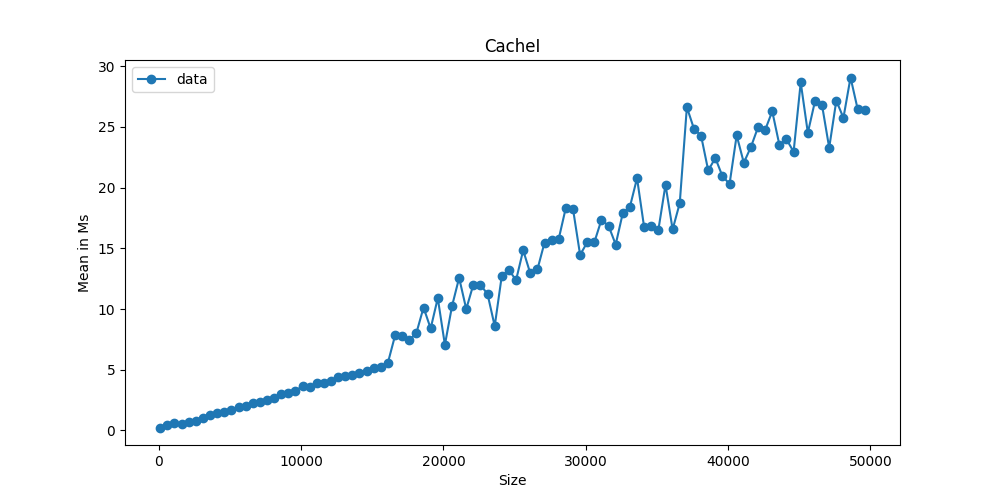
\includegraphics[width=0.9\linewidth]{images/cache_i_ms_50k_mean.png}
        \caption{Java implementation up to sizes of 50.000}
        \label{fig:image1}
    \end{minipage}\hfill
    \begin{minipage}{0.49\textwidth}
        \centering
        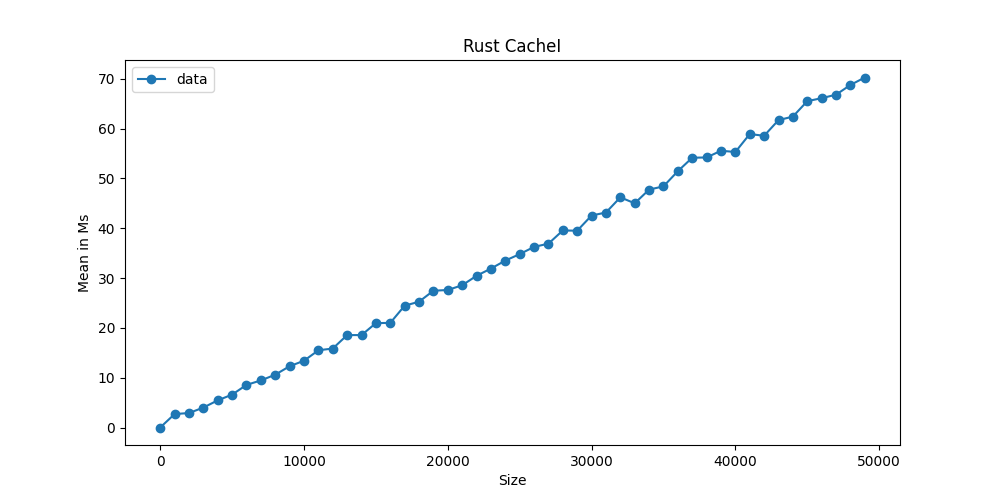
\includegraphics[width=0.9\linewidth]{images/cache_i_rs_mean.png}
        \caption{Rust implementation up to sizes of 50.000}
        \label{fig:image2}
    \end{minipage}
\end{figure}

Due to this reason, I decided that in this report I will go with the \emph{two pointers}
version, since java is delivering consistent data for this. But as a downside, it is of course way
worse when it comes to growth rates so I will only be able to run the benchmarks with sizes up to $5.000$
in steps of 100 with 20 repetitions, otherwise these would take way to long. To my discontent, the two pointer version
is as bad as the brute force version when it comes to duplication of already found triples, something that
was often halfed in the improved cached version, without duplication checking. I did not add any checking for 
duplicates in any implementation since that would just mean an increase in runtime and possibly scewing of the benchmarks.

\subsubsection{Two Pointers}

The two pointer implementation was the most verbose out of all of the algorithms. It is based on
two pointers that are moving from opposite sites of the list and eventually meet somewhere in the list.
It is required that the list is sorted for this to work, which adds more complexity and time to the algorithm.
Sorting a list, if a proper algorithm is used, has an $O(N log N)$ time complexity. 
The outer for loop  and the inner while loop combined with \emph{O(N)} each will combined result in 
$O(N^2)$. The all the operations within the loops, such as if statements and array indexing can be ignored.
This will leave us with $O(N log N) + O(N^2)$, but since $O(N^2)$ dominates in this case,
the total time complexity of this algorithm will be $O(N^2)$.

\pagebreak
\subsection{Problem 7 - Threesum Benchmarking \& Growth}

As mentioned in the preivous section, for this algorithm, the maximum sizes we are able to test it at 
are significantly lower than for the union find. So in this case, the tests were run for ranges from
100 to 5000 with steps of 100. As samples, I took 1, 2, 3 and 4 thousand. And to my pleasant surprise, even
just taking such a small amount of values was enough for quite accurate values.

\begin{table}[h]
    \centering
    \caption{\small{All the results of calculations based on the \emph{size} and \emph{time}. \emph{l2 t} = \emph{$log_2 time$}, \emph{l2 r} = \emph{$log_2 ratio$}}}
    \begin{tabular}{|c|c|c|c|c|c|c|c|}
        \hline size &	time &	l2t &	ratio &	l2r &	slope &	b &	c \\
        \hline 1000 &	186.63 &	7.54 &	N/A &	N/A &	N/A &	N/A &	N/A \\
        \hline 2000 &	749.74 &	9.55 &	4.02 &	2.01 &	5.6311e-01 &	2.006 &	-12.45 \\
        \hline 3000 &	1864.80 &	10.86 &	2.49 &	1.31 &	1.1151e+00 &	2.247 &	-15.09 \\
        \hline 4000 &	3408.16 &	11.73 &	1.83 &	0.87 &	1.5434e+00 &	2.096 &	-13.35 \\
        \hline average &	& 10.72 &	2.78 &	1.40 &	1.07e+00 &	2.117 &	-13.63 \\
        \hline
    \end{tabular}
\end{table}

Using the \emph{b (2.117)} and \emph{c (-13.63)} to create the power law results in the following.
a = 7.89e-5 = 0.0000789, b = 2.117, power law: $7.889e-05x^2.117$. We can then again use those numbers
to approximate the time for any size and get fairly accurate results.

\begin{minipage}{0.48\textwidth}
    \begin{tabular}{|c|c|c|c|}
        \hline size & original & pred & acc \\
        \hline 1000 & 186.63 & 176.46 & 1.06 \\
        \hline 2000 & 749.74& 765.21 & 0.98 \\
        \hline 3000 & 1864.80& 1805.03 & 1.03 \\
        \hline 4000 & 3408.16& 3318.35 & 1.03 \\
        \hline
    \end{tabular}
    \captionof{table}{\small{power law predictions vs \linebreak original time}}
\end{minipage}
\begin{minipage}{0.48\textwidth}
    \begin{tabular}{|c|c|c|c|}
        \hline size & original & pred & acc \\
        \hline 1000 & 7.54& 7.46 & 1.01 \\
        \hline 2000 & 9.55& 9.58 & 0.99 \\
        \hline 3000 & 10.86 & 10.82 & 1.00 \\
        \hline 4000 & 11.73& 11.70 & 1.00 \\
        \hline
    \end{tabular}
    \captionof{table}{\small{model predictions vs \linebreak original $log_2 time$}}
\end{minipage}

To determine the growth rate of the two pointers algorithm we can look at the \emph{b} value.
In this case it is around \emph{$2.1$}. While the quick find around 1 indicates linear growth and the 
sub 1 \emph{b} of the weighted quick union implementation indicated logarithmic/sublinear rates, an exponent b
of two suggests a quadratic growth, meaning the bigger the input size, the steeper the slope.
This however confirms our expectation of a quadratic growth rate and therefore should qualify
as a threesum that has an upper bound of $O(N^2)$.

In order to ensure that the the two pointer implementation actually has an upper bound of $O(N^2)$
I compared it to both my original cached version, which consists of two for loops and keeps track of a set, 
therefore being $O(N^2)$ and the improved cached version, both of which have a time complexity of $O(N^2)$.

\begin{figure}[h]
        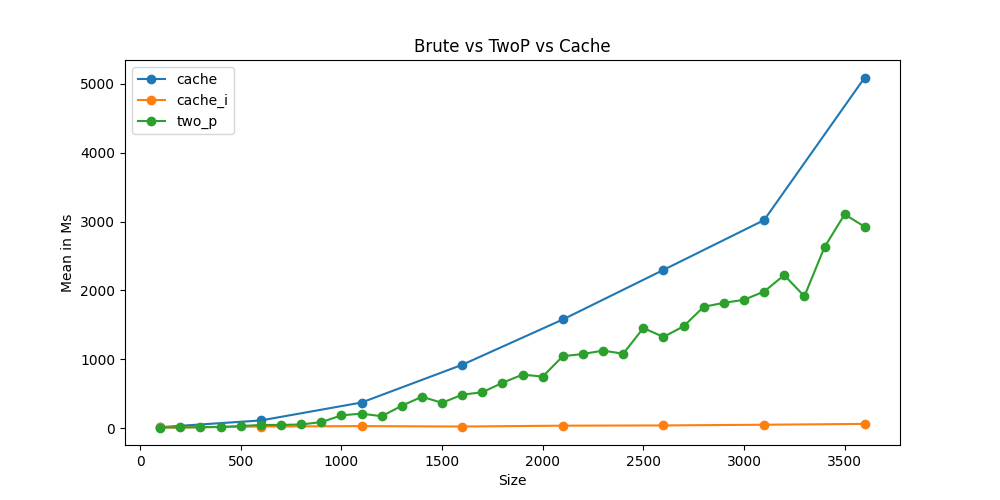
\includegraphics[width=0.9\linewidth]{images/comparison.png}
        \caption{Comparison between implementations}
        \label{fig:image1}
\end{figure}

As can be observed in the diagram, the two pointer implementation lies right in between the two cache implementations,
leading us to the confirmation that it has both a $\Omega{(N^2)}$ as well as an $O{(N^2)}$.

\section{Problems - VG}

\subsection{Problem 8 - Percolation}

In this section I will quickly go over how I implemented problem 8 and then tested it as well
as my approach for determining \emph{p*}.

\subsubsection{Implementation}

The main two components of my implementation are a \emph{n * n} zeroed grid (int[]) and one of the
union find implementations, in my case the weighted quick union find with path compression.
As already alluded to in the task description, when instantiating the union find object, instead of initiating
it just with \emph{$n^2$}, we add two more sites to it, so called virtual sites. One will serve
as the top and the other as the bottom site. Meaning that all the grid values are being stored from
0 to n - 1 and the top value will be $n^2$ and the bottom $n^2 + 1$.

The two crucial methods will be the \emph{open} and \emph{percolates} method. While the \emph{percolates}
method is simply calling the union finds \emph{connected} function with the top and bottom value to check if
there is a valid path through the grid, the open method is a bit more complex. After validating that
the row and column are indeed valid to be inserted and the site they describe is not already open, we open the 
site by setting it to 1 and increasing the internal tracker of how many sites are already open.
In order to connect new opened sites now, we check all fields horizontally and vertically adjacent
to it. If the site is also open, we call the \emph{union} method of the union find on both points.

\subsubsection{Testing}

In order to make sure that the implementation was working, I created a simple \emph{4x4} grid
and opened specific fields manually in a way that I knew they had to make the grid percolating.
This confirmed that what I had done worked correctly so I could move on to calculating the threshold.

\subsubsection{Calculating threshold}

For the calculation of the \emph{p} threshold I, as suggested, made use of the \emph{monte carlo}
approach. This quite frankly means, taking randomly generated input to approximate a value, that could have been
deterministically evaluated, but might take a lot of effort and time. In our case, that means
initialising an \emph{Percolation} instance for a size \emph{n}, and randomly opening a site
until the grid percolates. The number of trials in this case is simply \emph{$n^2$}. This is done multiple times,
in this case 500 times, after which the average is taken and those results used to calculate the 
standard deviation. This was done for 250 \emph{n's} ranging from 2 to 500. This resulted in a
final result of \emph{p* = 0.59191} with a standard deviation of \emph{std\_dev = 0.01261}.

\end{document}
